\chapter{Features}
In dit hoofdstuk wordt bestaande literatuur voor actieherkenning verkent en besproken. De voornaamste methoden maken enerzijds gebruik van kleurenbeelden \cite{Laptev2005}, \cite{Dollar2005}, \cite{Willems2008}, \cite{Wang2011} en anderzijds van dieptebeelden \cite{Li2010}, \cite{Wang2012a}, \cite{Xia2012}, \cite{Gu2010}. Onafhankelijk van welke beelden die gekozen worden, moeten er features geëxtraheerd worden. Volgende sectie bespreekt kort de voornaamste manieren om features te bepalen uit zowel kleuren- als dieptebeelden.
\section{Features uit kleurenbeelden}
In het geval van kleurenbeelden kan het bepalen van features in twee categorieën onderverdeeld worden: \textit{globale feature extraction} en \textit{lokale feature extraction} \cite{Poppe2010}. Bij een globale aanpak wordt een persoon eerst gelokaliseerd met behulp van background subtraction of tracking gevolgd door het encoderen van de interesseregio's. Deze representatie kan veel informatie bevatten, maar door de nood aan background subtraction of tracking is deze methode gevoelig aan ruis.

Een lokale aanpak tracht deze problemen te vermijden door eerst lokale interessepunten, in de literatuur \gls{ac:stip} genoemd, te bepalen. Deze interessepunten kunnen zowel het temporale als het ruimtelijke aspect modelleren. Rond deze interessepunten worden patches berekent, afhankelijk van gekozen parameters. De verzameling van zulke patches is de representatie. Deze methode geniet de voorkeur omdat background subtraction of tracking niet strikt noodzakelijk is zodat het minder gevoelig is aan ruis.
 
feature detectors:
\todo{harris3D \cite{Laptev2005}}
\todo{cuboid \cite{Dollar2005}} 
\todo{Hessian \cite{Willems2008}}
\todo{dense trajectory \cite{Wang2011}}

feature descriptors:
\todo{cuboid descriptor: \cite{Dollar2005}}
\todo{hog/hof \cite{Laptev2005}}
 
\section{Features uit dieptebeelden}
De methoden die bruikbaar zijn op kleurenbeelden zijn niet bruikbaar op dieptebeelden. Recente literatuur over feature extraction op dieptebeelden levert vaak algoritmen \cite{Xia2012}, \cite{Wang2012b}, \cite{Yang2012} op die gebruik maken van skeletbeelden gegeneerd met methode \cite{Shotton2011} waarop de skelettracker van de Kinect op gebaseerd is. De skeletbeelden van de Kinect geven de drie-dimensionale coördinaten van 25 punten, \textit{joints} genoemd, die belangrijke kenmerken van het menselijk lichaam voorstellen \todo{figuur van de joints}. Zo een skelettracker neemt de taak van een feature detector op zich, zodat algoritmen die gebruik maken van skeletbeelden enkel feature descriptors moeten implementeren. Deze joints bevatten echter geen temporale informatie zodat dit op een andere manier moet gemodelleerd worden. Vaak gebruikte modellen zijn \gls{ac:hmm} (\cite{Xia2012}, \cite{Gu2010}),  \gls{ac:crf} (\cite{Han2010}), \gls{ac:dtw} (\cite{Muller2006}) en \gls{ac:ftp} (\cite{Wang2012b}). Al deze modellen zijn temporale classifiers en worden kort besproken in sectie \ref{subsec:temporale_modellen}.

Het gebruik van de Kinect is geen vereiste om actieherkenning met dieptebeelden uit te voeren. \cite{Li2010} stelt elke frame voor als een verzameling van 3D punten, geëxtraheerd uit de silhouetten dat de dieptebeelden geven en maken gebruik van een \gls{ac:hmm} om het temporale aspect te modelleren. \cite{Wang2012a} 

In volgende onderdelen worden een aantal belangrijke feature descriptors beschreven.
\subsection{Histograms of 3D Joints (HOJ3D)}
Het werk van \cite{Xia2012} toont aan hoe een histogram van drie-dimensionale punten aan real-time actieherkenning kan doen. Ze transformeren het skeletbeeld gegenereerd door de Kinect om in bolcoördinaten. Als oorsprong wordt de heup joint genomen. De horizontale referentievector $\textbf{\alpha}$ wordt parallel met de grond genomen door de oorsprong. De verticale referentievector $\textbf{\theta}$ staat loodrecht op $\textbf{\alpha}$ en gaat ook door de oorsprong. De drie-dimensionale ruimte wordt opgesplitst in $84$ deelruimten. Elke joint zal zich dan in één van die 84 deelruimte bevinden. Een histogram wordt opgemaakt door elke joint te wegen in 8 naburige deelruimten via een Gaussische functie:

$$p(X, \mu, \Sigma) = \frac{1}{(2\pi)^{n/2}|\Sigma|^{1/2}}e^{-\frac{1}{2}(X - \mu)^T\Sigma^{-1}(X - \mu)}$$

Hierbij is $\mu$ de mediaanvector en $\Sigma$ de identiteitsmatrix. Voor zowel $\textbf{\Theta}$ als $\textbf{\alpha}$ wordt de kansfunctie apart uitgerekend. Stel $\Omega$ de cumulatieve distributiefunctie van de normaalverdeling, dan wordt de kans dat een joint met locatie $(\mu_\alpha, \mu_\theta)$ 

$$p(\theta_1 < \theta < \theta_2; \mu_\theta, \sigma) = \Omega(\theta_2; \mu_\theta, \sigma) - \Omega(\theta_1; \mu_\theta, \sigma)$$

$$p(\alpha_1 < \alpha < \alpha_2; \mu_\alpha, \sigma) = \Omega(\alpha_2; \mu_\alpha, \sigma) - \Omega(\alpha_1; \mu_\alpha, \sigma)$$

Dit levert de \gls{ac:hoj} descriptor op.



\subsection{Covariance Descriptors on 3D Joint Locations (COV3DJ)}
De methode van \cite{Hussein2011} maakt gebruik van covariantiematrices. Een covariantiematrix voor een verzameling van $N$ willekeurige variabelen is een $N \times N$ matrix waarvan de elementen de covariantie bevatten tussen elk paar variabelen. Als $\textbf{X} = (X_1, X_2, ..., X_N)$, een vector met $N$ random variabelen, dan wordt de covariantiematrix $K_{X_{i}X_{j}}$ gedefinieerd als:

$$K_{X_{i}X_{j}} = E[(X_i - E[X_i])(X_j - E[X_j])]$$

Zo een matrix bevat informatie over de gezamenlijke kans $P(X_j) \cdot P(X_i | X_j)$. Het eerste gebruik van zo een matrix is in het werk van \cite{Tuzel2006} met als doel een regio van een afbeelding te beschrijven.

Elke joint $i$ kan voorgesteld worden door zijn drie-dimensionale coördinaten voor een frame $t$: $p_i^{(t)} = (x_i^{(t)}, y_i^{(t)}, z_i^{(t)})$. De concatenatie van alle joints voor frame $t$ is een vector $\textbf{S}$, met $3K$ elementen: $\textbf{S} = (x_1, ..., x_K,y_1, ..., y_K,z_1, ..., z_K)$, hierbij is $K$ het aantal joints dat beschikbaar is op één frame. Voor $\textbf{S}$ zou nu de covariantiematrix berekent worden, maar de kansverdeling is niet gekend, zodat de steekproefcovariantie wordt gekozen. De resulterende matrix is symmetrisch ten opzichte van de hoofddiagonaal, zodat enkel de bovendriehoek moet beschouwd worden. Voor $K = 25$ is het aantal resulterende elementen in de bovendriehoek gelijk aan $2850$. In vergelijking met \cite{Hussein2011} waarbij ze $K = 20$ nemen, is het resultaat $1830$. Vijf extra joints zorgt al voor een toename van 1020 elementen in de matrix.

Deze descriptor, \gls{ac:cov3dj} genoemd, bevat de locaties van de verschillende joints, afhankelijk van elke andere joint tijdens een actie. De temporale informatie wordt beschreven als een hiërarchie van zulke descriptors. Het niveau $l$ duidt de diepte in de hiërarchie aan met $l = 0$ de top van de hiërarchie. Elk niveau bevat $2^l - 1$ descriptors die elk $\frac{T}{2^l}$ frames bevatten van de sequentie. Voor $l = 1$ zullen er drie descriptors gegenereerd worden die elk $T/2$ frames zullen modelleren waarbij $T$ het totaal aantal frames is. Dit wordt grafisch weergegeven op figuur \ref{fig:temporal_evolution_cov3dj}.

\begin{figure}
	\centering
	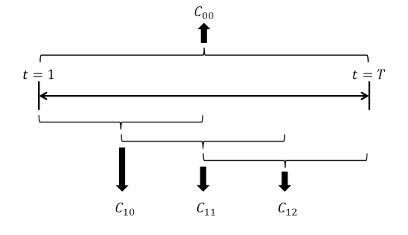
\includegraphics[width=0.5\textwidth]{temporal_evolution_cov3dj}
	\caption{De temporale constructie van de descriptor. $C_{li}$ is de $i$-de descriptor op niveau $l$. }
	\label{fig:temporal_evolution_cov3dj}
	\source{Figuur 2 in \cite{Hussein2011}.}
\end{figure}

Elke descriptor op elk niveau bevat nog steeds hetzelfde aantal elementen ($1830$ voor $K = 20$ of $2850$ voor $K = 25$), zodat de lengte van de totale descriptor nu gelijk is aan het aantal descriptors maal het aantal elementen. Voor $K = 20$ en $K = 25$ bedraagt de lengte voor figuur \ref{fig:temporal_evolution_cov3dj} respectievelijk $7320$ en $11\,400$.

\subsection{Local Occupancy Pattern (LOP)}
Deze methode \cite{Wang2012b} berekent allereerst de drie-dimensionale afstand van elke joint $i$ tot elke andere joint $j$: $\textbf{p}_{ij} = \textbf{p}_i - \textbf{p}_j$. De feature vector voor elke joint $i$ wordt dan:
$$\textbf{p}_i = \{\textbf{p}_{ij} | i \neq j \}$$

Aanvullend aan deze feature wordt een \gls{ac:lop} gedefinieerd. Deze feature geeft de lokale bezettingsgraad aan; een maat om aan te geven in hoeverre een joint door een ander object gehinderd wordt. Op frame $t$ wordt er een puntenwolk gegenereerd op basis van het dieptebeeld. Voor elke joint $j$ wordt zijn lokale regio gepartitioneerd in een $N_x \times N_y \times N_z$ raster. Elke cel van dit raster bevat $S_x \times S_y \times S_z$ pixels. Voor elke cel $c_{xyz}$ wordt de som van de punten genomen die zich in die cel bevinden. De sigmoïdefunctie $\delta(x) = \frac{1}{1 + e^{-\beta x}}$ wordt toegepast op deze som om zo de feature $o_{xyz}$ te bekomen:

$$o_{xyz} = \delta\bigg(\sum_{q \in c_{xyz}} I_q \bigg)$$
\subsection{EigenJoints}
Het werk van \cite{Yang2012} introduceert een nieuwe soort joint, de \textit{EigenJoint}. Ze maken gebruik van de drie-dimensionale positieverschillen tussen elk paar van joints en extraheren drie features voor elke frame $c$: de \textit{posture feature} $f_{cc}$, de \textit{motion feature} $f_{cp}$ en de \textit{offset feature} $f_{ci}$. Deze drie features worden geconcateneerd om de feature $f_c = (f_{cc}, f_{cp}, f_{ci})$ te bekomen. Deze feature wordt genormaliseerd via \gls{ac:pca}. Elke frame $i$ bevat $N$ joints: $X_i = \{x_1^i, x_2^i, ..., x_N^i \}$

De \textit{posture feature} beschrijft de statische postuur dat een persoon aanneemt. Voor elke joint wordt de drie-dimensionale afstand berekent tussen elk paar van joints voor de huidige frame $c$:
$$f_{cc} = \{x_i^c - x_j^c | i , j = 1, 2, ..., N; i \neq j\}$$
De dynamiek wordt gemodelleerd met de \textit{motion feature} die de drie-dimensionale afstand berekent tussen elke joint van de huidige frame $c$ met elke andere joint van de vorige frame $p$: 
$$f_{cp} = \{x_i^c - x_j^p | x_i^c \in X_c ; x_j^p \in X_p \}$$

Tot slot wordt nog de \textit{offset feature} gedefinieerd, die de algemeen dynamiek modelleert door de drie-dimensionale afstand te berekenen tussen elke joint van de huidige frame $c$ met elke andere joint van de initiële frame $i$:
$$f_{ci} = \{x_i^c - x_j^i |  x_i^c \in X_c ; x_j^p \in X_i \}$$

De verzameling van deze drie feature vectoren wordt $f_c$ genoemd. Er wordt een lineaire normalisatie uitgevoerd zodat elk attribuut in $f_c$ zich in het bereik $[-1, +1]$ bevindt zodat $f_{norm}$ bekomen wordt. Het aantal dimensies wordt vrij hoog; voor $N = 25$ zorgen $f_{cc}$, $f_{cp}$ en $f_{ci}$ respectievelijk voor $300$, $625$ en $625$ jointbewerkingen op. Elke bewerking genereert drie attributen, $\delta x, \delta y, \delta z$, zodat de totale dimensie van $f_c$ gelijkgesteld moet worden aan $ (300 + 625 + 625) \times 3 = 4650$. In vergelijking met \cite{Yang2012} waarbij ze $N = 20$ gebruiken, is de totale dimensie $2970$.


\chapter{Classificatie}
Op het moment dat een feature vector opgebouwd is voor een individuele frame of een verzameling van frames is het actieherkenningprobleem gereduceerd tot een classificatieprobleem. De bekomen feature vector wordt als input aan een classifier gegeven die dan tracht de juiste klasse toe te kennen op basis van de leerverzameling. Voor actieherkenning kunnen drie algemene methoden beschreven worden:
\begin{enumerate}
	\item Classificeren zonder de temporale dimensie expliciet te modelleren, \textit{directe classificatie};
	\item Classificeren waarbij de temporale dimensie wel gemodelleerd wordt, \textit{temporale modellen};
	\item Algemene classificatie zonder de actie te modelleren, \textit{actiedetectie}.
\end{enumerate}

\section{Directe classificatie}
Wanneer het temporale aspect verworpen wordt zijn er maar twee mogelijkheden: alle geobserveerde frames vervatten in één enkele representatie of actieherkenning uitvoeren op elke individuele frame. Een voorbeeld van zo een algoritme is $k$-nearest neighbours. Deze methode maakt gebruik van de afstand van de geobserveerde feature vector tot elke andere feature vector uit de leerverzameling. Uit de $k$ dichtste buren wordt dan de klasse genomen die het meest voorkomt. Deze operatie vraagt voor een grote leerverzameling veel rekenkost omdat elke feature vector gecontroleerd moet worden. Deze methode kan zowel op frame-niveau als op sequentieniveau werken. In het tweede geval wordt er met bijvoorbeeld majority voting de klasse gekozen die het meest voorkomt in een sequentie van frames.


\section{Temporale modellen}
\label{subsec:temporale_modellen}
Bij temporale modellen zijn er twee grote klassen te onderscheiden: \textit{generatieve} en \textit{discriminerende} modellen. Een generatief algoritme modelleert hoe een input $x$ wordt gegenereerd om zo een actieklasse $y$ toe te kennen en maakt gebruik van de gezamenlijke kansverdeling $P(x, y) = P(x|y)P(y)$. Een generatief model zal dus de kansverdeling van de leerverzameling modelleren en zal bij een nieuwe observatie. Een discriminerend model zal de kans $P(y|x)$ direct modelleren zodat een directe mapping van $x$ op $y$ beschikbaar is. De onderliggende kansverdelingen worden dan ook niet berekent.
 
Er bestaat een grote discussie over welk van deze twee modellen nu de voorkeur krijgen. Er is aangetoond \cite{Andrew2002} dat discriminerende modellen de voorkeur genieten.

\subsection{Generatieve modellen}

Een \gls{ac:hmm} is een typisch voorbeeld van een generatief model. Een \gls{ac:hmm} is een uitbreiding van een Markov model waarbij de staat van elke toestand nu verborgen is. De toestanden zijn hier de verschillende fasen van een bepaalde actie. Een \gls{ac:hmm} gaat uit van twee assumpties:
\begin{enumerate}
	\item Een verandering van toestand hangt enkel af van de vorige toestand. Dit wordt ook de \textit{Markov eigenschap} genoemd.
	\item De observatie behorend bij een toestand is onafhankelijk van elke andere observatie.
\end{enumerate}

Voor een verzameling met $n$ klassen $\Lambda = \lambda^1 ... \lambda^n$ en een verzameling met $k$ observaties $O = \{o_1 ... o_k\}$, moet de juiste klasse $\lambda$ geselecteerd worden die de kans op $P(\lambda | O)$ maximaliseert.

$$\lambda = \arg\max_{\substack{1 \leq i \leq n}} P(O|\lambda^i) $$


\subsection{Discriminerende modellen}
\subsubsection{Conditional Random Fields}
Een \gls{ac:hmm} gaat ervan uit de observaties onafhankelijk zijn van elkaar, wat niet altijd het geval is. Een \gls{ac:crf} is een voorbeeld van een discriminerend model. Een discriminerende classifier houdt rekening met meerdere observaties in de tijd en is geschikt voor de classificatie van een reeks van observaties. Een \gls{ac:crf} gaat ervan uit dat de volgorde van observaties wel degelijk een impact heeft op de betekenis van deze observaties.

\subsubsection{Dynamic Time Warping}
\gls{ac:dtw} is een algoritme dat de gelijkenis tussen twee sequenties bestudeerd, die verschillend kunnen zijn in snelheid. In actieherkenning lost dit het probleem van verschillen in actiesnelheid op. Een persoon die trager of sneller zwaait dan een persoon in de leerverzameling, kan via \gls{ac:dtw} toch herkent worden. Veronderstel twee verzamelingen van feature vectoren $X = \{x_1, x_2, ... x_N\}$ en $Y = \{y_1, y_2, ..., y_M\}$, een kostfunctie $c(x, y)$ die de kost bepaald tussen twee feature vectoren en $p = \{p_1, ..., p_L\}$ met $p_l = (n_l, m_l)$  

Een \gls{ac:dtw} heeft bepaalde restricties:
\begin{itemize}
	\item $p_1 = (1, 1)$ en $p_L = (N, M)$.
	\item $n_1 \leq n_2 \leq ... \leq n_L$ en $m_1 \leq m_2 \leq ... \leq m_L$.
\end{itemize}


\section{Key frames}
In plaats van elke frame te classificeren, zou een actie kunnen voorgesteld worden door \textit{key frames}. Dit is een selectie van frames die een actie voldoende kunnen voorstellen zodanig dat verschillende acties nog steeds onderscheidbaar zijn en variaties van dezelfde actie hetzelfde gelabeld worden. In de literatuur bestaan er diverse manieren om zulke key frames te bepalen. De methode van \cite{Suolan2017} berekent een verschil op basis van de joints die de Kinect beschikbaar stelt. De methode van \cite{Carlsson2001} maakt gebruik van randdetectie om silhouette te bekommen en zoekt een match tussen voorgedefinieerde silhouetten die een key frame van een actie voorstelt. Andere methoden maken ook gebruik van voorgedefinieerde exemplaren \cite{Weinland2008a}, \cite{Fathi2007},
